% Created 2016-09-23 Fri 02:06
\documentclass[11pt]{article}
\usepackage[utf8]{inputenc}
\usepackage[T1]{fontenc}
\usepackage{fixltx2e}
\usepackage{graphicx}
\usepackage{longtable}
\usepackage{float}
\usepackage{wrapfig}
\usepackage{rotating}
\usepackage[normalem]{ulem}
\usepackage{amsmath}
\usepackage{textcomp}
\usepackage{marvosym}
\usepackage{wasysym}
\usepackage{amssymb}
\usepackage{hyperref}
\tolerance=1000
\author{anoop}
\date{\today}
\title{readme}
\hypersetup{
  pdfkeywords={},
  pdfsubject={},
  pdfcreator={Emacs 24.5.1 (Org mode 8.2.10)}}
\begin{document}

\maketitle
\tableofcontents

\section{FINITE ELEMENTS}
\label{sec-1}
\subsection{Introduction}
\label{sec-1-1}
The finite element method (FEM) is a numerical technique for finding approximate solutions to boundary value problems for partial differential equations. In other words it can be used to find solutions to problems that can be expressed into 'governing equations' and 'boundary conditions'.
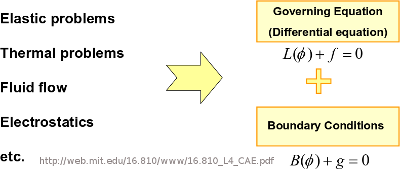
\includegraphics[width=4in]{images/fem.png}
One of the relatively easy problems to sole with FEM is the Poisson's problem, modeling the diffusion of temperature in a body. Which can be stated as follows. Given a domain $\Omega$ $\subset$ R$^{\text{2}}$

\subsection{Theory}
\label{sec-1-2}
% Emacs 24.5.1 (Org mode 8.2.10)
\end{document}
